%!TEX root = ..\..\..\..\Main.tex
\subsection{Kinect}
The Microsoft Kinect products are motion sensing devices equipped with depth sensors (using infrared technology) and ordinary color cameras.
Since the Emotiv EPOC signals scramble when the person blinks or moves his eyebrows, the idea for this fusion is to capture those motions in order to filter out the spikes in the EEG data that is found to be caused by blinking or eyebrow movement.
There are currently two variants, the Kinect v1 (used for Xbox 360, 2010) and the Kinect v2 (used for Xbox One, 2014).
Their specifications are listed in Table \ref{[KINECT] Specification Comparison}, however we only have V1 so this is the one we will be evaluating.

\begin{table}[H]
\centering
\caption{Kinect specification comparison\cite{kinect_specs1}\cite{kinect_specs2}\cite{kinect_specs3}\cite{kinect_specs4}.}
\label{[KINECT] Specification Comparison}
\begin{tabular}{r|
>{\columncolor[HTML]{FFE8E7}}c |	
>{\columncolor[HTML]{DCECFF}}c |}
\cline{2-3}
                 & \cellcolor[HTML]{FFCCC9}{\bf V1} & \cellcolor[HTML]{BBDAFF}{\bf V2} \\ \cline{2-3} 
Depth Resolution & 320 x 240                        & 512 x 424                        \\ \cline{2-3} 
Depth Framerate  & 30Hz                             & 30Hz                             \\ \cline{2-3} 
Color Resolution & 640 x 480                        & 1920 x 1080                      \\ \cline{2-3} 
Color Framerate  & 30Hz                             & 30Hz                             \\ \cline{2-3} 
Minimum Distance & 1.8m                             & 1.4m                             \\ \cline{2-3} 
\end{tabular}
\end{table}

Using the Kinect V1 and two demo softwares, Face Tracking 3d-WPF and Face Tracking Basics-WPF, from the Kinect Developer Tools, we captured three facial expressions for comparison.
The three facial expressions are:
\begin{itemize}
\item Open eyes, low brows
\item Closed eyes, low brows
\item Open eyes, raised brows
\end{itemize}

The results from \textit{Face Tracking 3d-WPF} show that it is difficult to capture the state of the eyes.
The eyes in Figure \ref{[KINECT][TEXTURED] Open eyes, low brows} and Figure \ref{[KINECT][TEXTURED] Closed eyes, low brows} are nearly indistinguishable.
The eyebrows, however, are easily distinguishable in Figure \ref{[KINECT][TEXTURED] Open eyes, low brows} and Figure \ref{[KINECT][TEXTURED] Open eyes, raised brows}.
The results from \textit{Face Tracking Basics-WPF} also show that raised eyebrows are better distinguished, than open/closed eyes.

\begin{figure}[H]
	\centering
	\begin{subfigure}{.3\textwidth}
		\centering
		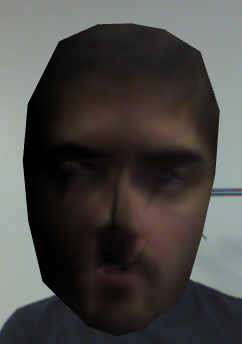
\includegraphics[width=0.8\linewidth]{sections/analysis/sensorselection/kinect/texture_no_face}
		\caption{Open eyes, low brows.}\label{[KINECT][TEXTURED] Open eyes, low brows}
	\end{subfigure}\hfill
	\begin{subfigure}{.3\textwidth}
		\centering
		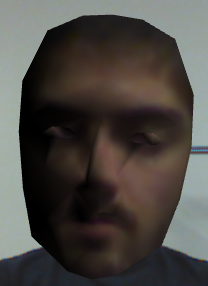
\includegraphics[width=0.8\linewidth]{sections/analysis/sensorselection/kinect/texture_closed_eyes}
		\caption{Closed eyes, low brows.}\label{[KINECT][TEXTURED] Closed eyes, low brows}
	\end{subfigure}\hfill%
	\begin{subfigure}{.3\textwidth}
		\centering
		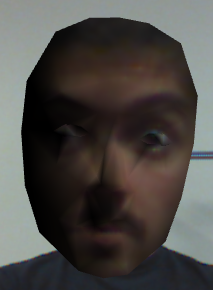
\includegraphics[width=0.8\linewidth]{sections/analysis/sensorselection/kinect/texture_brows_high}
		\caption{Open eyes, raised brows.}\label{[KINECT][TEXTURED] Open eyes, raised brows}
	\end{subfigure}
	\caption{Face Tracking 3d-WPF, Kinect V1.}
	\label{[KINECT][TEXTURED] Textured captures.}
\end{figure}

Since the average duration of an eye blink is between 0.1 seconds and 0.4 seconds\cite{eye_blink_duration} and the frequency of measurement of the Kinects are 30Hz, catching an eye blink should be possible.
It is possible that the V2 is better able to catch this, due to increased capture resolution and lower minimum distance to the face, both of which will result in a higher quality depth map.

\begin{figure}[H]
	\centering
	\begin{subfigure}{.3\textwidth}
		\centering
		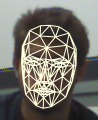
\includegraphics[width=0.8\linewidth]{sections/analysis/sensorselection/kinect/poly_noface}
		\caption{Open eyes, low brows.}\label{[KINECT][WIREFRAME] Open eyes, low brows}
	\end{subfigure}\hfill
	\begin{subfigure}{.3\textwidth}
		\centering
		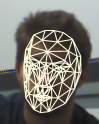
\includegraphics[width=0.8\linewidth]{sections/analysis/sensorselection/kinect/poly_closed_eyes}
		\caption{Closed eyes, low brows.}\label{[KINECT][WIREFRAME] Closed eyes, low brows}
	\end{subfigure}\hfill%
	\begin{subfigure}{.3\textwidth}
		\centering
		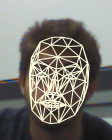
\includegraphics[width=0.8\linewidth]{sections/analysis/sensorselection/kinect/poly_brows_high}
		\caption{Open eyes, raised brows.}\label{[KINECT][WIREFRAME] Open eyes, raised brows}
	\end{subfigure}
	\caption{Face Tracking Basics-WPF, Kinect V1.}
	\label{[KINECT][WIREFRAME] Wireframe captures.}
\end{figure}